\documentclass[11pt]{book}

\usepackage{epsfig}
\usepackage{html}
\usepackage{hypre}
\usepackage{makeidx}
\usepackage{graphicx}

%=============================================================================
% Preamble:
%=============================================================================

% set margins
\setlength{\oddsidemargin}{0in}
\setlength{\evensidemargin}{0in}
\setlength{\textwidth}{6.5in}
\setlength{\topmargin}{0in}
\setlength{\textheight}{8.0in}

% define various commands and macros

% define the version number
% NOTE: this is automatically generated from another file in hypre
\input{version}

% write out the index entries in the `.idx' file
\makeindex

%=============================================================================
% Body:
%=============================================================================

\begin{document}

%=============== Title Page

\begin{TitlePage}

\Title{\hypre{} User's Manual: Draft}
\SubTitle{Software Revision: \HYPREVersion}
\SubTitle{Date: \HYPREVersionDate}
\vfill
\begin{center}
\InsertGraphics{hypre_wiw}{width=.7\textwidth}
\end{center}
\vfill
\Author{%
Center for Applied Scientific Computing\\
Lawrence Livermore National Laboratory
}

\end{TitlePage}

%=============== Copyright Page

\begin{CopyrightPage}

\noindent
Copyright \copyright{} 1998 The Regents of the University of California.

\vspace{1em}\noindent
Permission is granted to make and distribute verbatim copies of this
manual provided the copyright notice and this permission notice are
preserved on all copies.

\vspace{1em}\noindent
This work was produced at the University of California, Lawrence
Livermore National Laboratory (UC LLNL) under contract
no. W-7405-ENG-48 (Contract 48) between the U.S. Department of Energy
(DOE) and The Regents of the University of California (University) for
the operation of UC LLNL. The rights of the Federal Government are
reserved under Contract 48 subject to the restrictions agreed upon by
the DOE and University as allowed under DOE Acquisition Letter 97-1.

\vspace{1em}\noindent
This work was prepared as an account of work sponsored by an agency of
the United States Government. Neither the United States Government nor
the University of California nor any of their employees, makes any
warranty, express or implied, or assumes any liability or
responsibility for the accuracy, completeness, or usefulness of any
information, apparatus, product, or process disclosed, or represents
that its use would not infringe privately-owned rights.  Reference
herein to any specific commercial products, process, or service by
trade name, trademark, manufacturer or otherwise does not necessarily
constitute or imply its endorsement, recommendation, or favoring by
the United States Government or the University of California. The
views and opinions of authors expressed herein do not necessarily
state or reflect those of the United States Government or the
University of California, and shall not be used for advertising or
product endorsement purposes.


\vspace{1em}\noindent
UCRL-MA-137155 DR
\end{CopyrightPage}

%=============== Table of Contents

\pagenumbering{roman}
\tableofcontents
\cleardoublepage
\pagenumbering{arabic}

%=============== Include Chapters

%==========================================================================
\chapter{Introduction}
\label{Introduction}

\hypre{} is a software library focused on the solution of large, sparse linear
systems of equations on highly parallel distributed-memory computer
systems. The library has been created with the goals of robustness,
computational performance, ease of use, flexibility, and interoperability
with other similar libraries. The mathematical emphasis is to provide
the latest scalable preconditioner algorithms to application codes
with a minimum of delay between development and deployment.

\section{Overview}

The following is a high-level list of the major features, assumptions and
limitations, and modes of use of 
\hypre{}. All of these subjects will be discussed in more detail later in this
User's Guide.

\subsection{Features}

\begin{itemize}

\item
{\bf Scalable Preconditioners Provide Efficient Solution on Today's and Tomorrow's
Systems:} \hypre{} 
contains several families of complex preconditioner algorithms focused on the
scalable solution of very 
large sparse linear systems. \hypre{} includes algorithms that other
general-purpose libraries cannot, such as 
structured multigrid, through the use of the Grid-centric interfaces discussed
below. These interfaces 
provide more information to solvers than traditional sparse matrix data
structures can provide, enabling 
more effective algorithms.

\item
{\bf Suite of Common Iterative Methods Provides Options for a Spectrum of Problems:}
\hypre{} provides 
an assortment of the most widely used Krylov-based iterative methods to be used
in conjunction with the 
scalable preconditioners. This includes general methods such as GMRES and
methods specialized for 
symmetric matrices such as Conjugate Gradient.

\item
{\bf Intuitive Grid-Centric Interfaces Obviate Need for Complex Data Structures:}
\hypre{} has made a 
major step forward in usability from earlier generations of sparse linear
solver libraries in that users do not 
have to learn complicated sparse matrix data structures. Instead, \hypre{} does
the work of building these 
data structures for the user through a variety of interfaces, each appropriate
to different classes of users. 
These include a structured, stencil-based interface most appropriate for
finite-difference applications; an 
unstructured finite-element based interface; and a linear-algebra based
interface. Other interfaces will be 
added as time and demand dictate.
Each interface provides access to several solvers without the need to
write new interface code.

\item
{\bf Many User Options Accommodate Beginners through Experts:} \hypre{} allows a
spectrum of expertise 
to be applied by users. The beginning user can get up and running with a
minimal amount of effort. More expert users can take further
control of the solution process 
through various parameters, all of which have reasonable defaults. 
%Further expertise can 
%allows users to put together their own solvers using components of \hypre{} as
%"building blocks", a 
%technique enabled through a new, flexible object model for linear solver
%libraries.

\item
{\bf Many Configuration Options to Suit your Computing System:} \hypre{} utilizes the
autoconf package to 
allow simple and flexible installation on a wide variety of computing systems.
Users can tailor the 
installation to match their computing system. Options include debug and
optimized modes, modes for 
including components from other installed linear solver libraries such as PETSc
and ISIS++ (see below), 
the ability to change dependent libraries such as MPI and BLAS, a
serial-machine mode, and modes 
enabling threads for certain solvers. On most systems, however, \hypre{} can be
built by simply typing 
"configure" followed by "make".

\item
{\bf Compatibility/Interoperability with Other Libraries Allows Plug and Play with
and Importing from 
other major solver libraries:} \hypre{} has been co-designed with the Equation
Solver Interface forum, a 
consortium of developers of sparse linear system libraries. The goal of the
forum is to design standard 
interfaces for these libraries that allow them to be compatible and
interoperable with each other. This 
process is ongoing, but it already allows \hypre{} users to invoke solvers and
preconditioners from libraries 
such as PETSc, ISIS++, and Aztec, oftentimes mixing and matching elements from
one library with 
elements from another. This provides a huge increase in options for users so
that they can find the unique 
combination that works best for them.

\item
{\bf Interfaces in Multiple Languages Provide Greater Flexibility for Applications:}
\hypre{} contains 
interfaces for both Fortran and C users.
%another major breakthrough in flexibility and usability: it is callable from a
%wide variety of languages. We 
%have used the Babel project to provide interfaces in C, C++, and Fortran, and
%as Babel adds support for 
%other languages, those languages will be added to \hypre{}. Babel allows \hypre{} to
%use an object-oriented 
%design in each of the supported languages, thus eliminating the need for \hypre{}
%to be written to the so-
%called "lowest common denominator".

\end{itemize}

\subsection{Assumptions and Limitations}

{\bf \hypre{} is designed for large, sparse, linear systems on parallel
computers.}  Small linear systems, 
systems that are solvable on a sequential computer, and dense systems are all
better addressed by libraries designed specifically for them. 

{\bf \hypre{} requires an installation of the Message Passing Interface (MPI).}
Exception: will run 
sequentially (for debugging) with an included "stub" version of MPI.

{\bf Configuration of \hypre{} with threads
requires an implementation of the Open MP standard.}
Only a small set of \hypre{} is compatible with threads at the current time.

{\bf Configuration of \hypre{} with other libraries requires installation of and
linking to those libraries.}

{\bf \hypre{} is a project under construction.} Systems problems, SAMR interface,
semi-structured interface, 
AMGe, full object orientation, full multilanguage support, ESI not integrated
yet, etc.




\section{General Structure of Usage}

Give example code here, maybe Rob's structured example is clearest. Use it to
demonstrate basic structure of usage:  This be temporarily yucky -MAL

\begin{display}
\begin{verbatim}

/*-----------------------------------------------------------
 * Set up the matrix
 *-----------------------------------------------------------*/

   HYPRE_StructGridCreate(MPI_COMM_WORLD, dim, &grid);

   /* Use HYPRE_StructGridSetExtents to define size in index space of
      each grid block making up the grid */

   HYPRE_StructGridSetPeriodic(grid, periodic);
   HYPRE_StructGridAssemble(grid);
	
   HYPRE_StructStencilCreate(dim, dim + 1, &stencil);

   /* Use HYPRE_StructStencilSetElement to impart structure to stencil */

   HYPRE_StructMatrixCreate(MPI_COMM_WORLD, grid, stencil, &A);

   /* Use grid and stencil to set matrix structure on matrix creation */

   HYPRE_StructMatrixSetSymmetric(A, 1);
   HYPRE_StructMatrixSetNumGhost(A, A_num_ghost);
   HYPRE_StructMatrixInitialize(A);

   /* Use HYPRE_StructMatrixSetBoxValues to set coefficients
      of matrix A */

   HYPRE_StructMatrixAssemble(A);

/*-----------------------------------------------------------
 * Set up the right-hand side and initial guess
 *-----------------------------------------------------------*/

   HYPRE_StructVectorCreate(MPI_COMM_WORLD, grid, stencil, &b);
   HYPRE_StructVectorInitialize(b);

   /* Use HYPRE_StructVectorSetBoxValues to set values of
      right-hand side b */

   HYPRE_StructVectorAssemble(b);

   HYPRE_StructVectorCreate(MPI_COMM_WORLD, grid, stencil, &x);
   HYPRE_StructVectorInitialize(x);

   /* Use HYPRE_StructVectorSetBoxValues to set values of
      initial guess x */

   HYPRE_StructVectorAssemble(x);

/*-----------------------------------------------------------
 * Set up solver
 *-----------------------------------------------------------*/

   HYPRE_StructPFMGCreate(MPI_COMM_WORLD, &solver);

/* Set solver parameters */
   HYPRE_StructPFMGSetMaxIter(solver, 50);
   HYPRE_StructPFMGSetTol(solver, 1.0e-06);
   HYPRE_StructPFMGSetRelChange(solver, 0);
   HYPRE_StructPFMGSetRelaxType(solver, 1);
   HYPRE_StructPFMGSetNumPreRelax(solver, n_pre);
   HYPRE_StructPFMGSetNumPostRelax(solver, n_post);
   HYPRE_StructPFMGSetSkipRelax(solver, skip);
   HYPRE_StructPFMGSetLogging(solver, 1);

   HYPRE_StructPFMGSetup(solver, A, b, x);

/*-----------------------------------------------------------
 * Solve the linear system
 *-----------------------------------------------------------*/

   HYPRE_StructPFMGSolve(solver, A, b, x);

/*-----------------------------------------------------------
 * Get solver results
 *-----------------------------------------------------------*/

/* Get solver statistics */
   HYPRE_StructPFMGGetNumIterations(solver, &num_iterations);
   HYPRE_StructPFMGGetFinalRelativeResidualNorm(solver, &final_res_norm);

/* Get solution */
  /* Use HYPRE_StructVectorGetBoxValues to get solution into simple
     arrays */

/*-----------------------------------------------------------
 * Deallocate solver memory space 
 *-----------------------------------------------------------*/
   HYPRE_StructPFMGDestroy(solver);

/*-----------------------------------------------------------
 * Deallocate linear system memory space 
 *-----------------------------------------------------------*/
   HYPRE_StructGridDestroy(grid);
   HYPRE_StructStencilDestroy(stencil);
   HYPRE_StructMatrixDestroy(A);
   HYPRE_StructVectorDestroy(b);
   HYPRE_StructVectorDestroy(x);

\end{verbatim}
\end{display}


{\bf \it Before coding:}

\begin{enumerate}

\item
{\bf Choose a conceptual interface.} Generally, the choice is fairly obvious, as,
say, a structured grid 
interface is clearly inappropriate from an unstructured grid application. It is
desirable to use a more 
specific interface if appropriate, e.g., the linear-algebraic interface is
usable from any type of grid but 
will involve much more user work and prevent access to some grid-type-specific
preconditioners.

\item 
{\bf Choose a desired solver/preconditioner combination.} For the typical user,
this will mean a single 
Krylov method and a single preconditioner. Some common combinations have been
prewrapped as a 
single solver to make them easier to use. 
%More advanced users might choose to,
%say, use two 
%preconditioners, composed through residual correction, to create a more robust
%solution method.

\item 
{\bf Look up matrix requirements for each solver and preconditioner.} Each
specific solver and 
preconditioner ("Operator") has requirements from the input matrix. Some only
work with specific 
matrix types, while others can work with any matrix that provides certain
"services" (for example, 
most Krylov solvers only need a "matrix-vector" multiplication service from the
input matrix). This 
information is provided in several places (Developer's Guide, source comments,
headers) in the form 
of type information.

\item 
{\bf Choose a matrix class that is compatible with your solvers/preconditioners and your
conceptual 
interface.} This can be done by inspecting the documentation, or alternatively,
by running a small 
problem size, as compatibility is checked within \hypre{} at runtime and produces
an error condition 
(errors are discussed more fully later) if the types are found to be
incompatible.

\end{enumerate}

Once the previous set of decisions have been made, it is time to code your application 
to call HYRPE:

\begin{itemize}

\item
{\bf Build any necessary auxiliary structures for your chosen conceptual
interface.} This includes, e.g., 
the grid and stencil structures for the structured grid interface.

\item
{\bf Build the matrix and vectors through your chosen conceptual interface.} Each
conceptual interface 
provides a series of calls for entering information about your problem into
\hypre{}.

\item
{\bf Build solvers and preconditioners by giving them the input matrix.}

\item
{\bf Set solver parameters.} Some parameters like convergence tolerance are the
same across solvers, 
while others are solver specific.

\item
{\bf Call the solve function for the solver.}

\item
{\bf Retrieve desired information from solver.} Depending on your application,
there may be different 
things you may want to do with the solution vector. Also, performance
information such as number of 
iterations is typically available, though it may differ from solver to solver.

\end{itemize}


{\bf Note on capitalization:} We use \code{HYPRE} and \code{hypre }
to divide \hypre{}'s function
calls into two kinds: 
those supported for users, and internal function calls. Expert users are
welcome to dig into \hypre{} source 
code and use internal function calls if they want to, but we make no promise
that those functions are fully 
supported or fully tested, nor that they will not change in future releases of
\hypre{}. 



%==========================================================================
\chapter{Conceptual Interfaces for Inputting Problem Data}
\label{Conceptual Interfaces}

\section{What do we mean by ``conceptual interfaces?''}

In Figure \ref{fig-conceptual-interface} we present an illustration
of the philosophy behind conceptual interfaces.

%[Cut and paste from Rob's paper].

\begin{figure}
\centering
\includegraphics[width=5in]{concep_iface.eps}
\caption{%
Graphic illustrating the notion of conceptual interfaces.}
\label{fig-conceptual-interface}
\end{figure}

%\section{Which conceptual interface should I use?}


%==========================================================================
\chapter{Structured-Grid System Interface (Struct)}
\label{Structured-Grid System Interface}

In order to get access to the most efficient and scalable solvers for
scalar structured-grid applications, users should use the
\code{Struct} interface described in this chapter.  This interface
will also provide access (this is not yet supported) to solvers in
\hypre{} that were designed for unstructured-grid applications and
sparse linear systems in general.  These additional solvers are
usually provided via the unstructured-grid interface (\code{FEI}) or
the linear-algebraic interface (\code{IJ}) described in Chapters
\ref{Finite Element Interface} and \ref{Linear-Algebraic System Interface}.

Figure \ref{fig-fv-grid} gives an example of the type of grid
currently supported by the \code{Struct} interface.  The interface
uses a finite-difference or finite-volume style, and currently
supports only scalar PDEs (i.e., one unknown per gridpoint).
\begin{figure}[t]
\centering
\includegraphics[width=4in]{fv_grid.eps}
\caption{%
An example 2D structured grid, distributed accross two processors.}
\label{fig-fv-grid}
\end{figure}
There are four basic steps involved in setting up the linear system
to be solved:
\begin{enumerate}
\item set up the grid,
\item set up the stencil,
\item set up the matrix,
\item set up the right-hand-side vector.
\end{enumerate}
To describe each of these steps in more detail, consider solving the
2D Laplacian problem
\begin{equation}\label{eqn-laplacian}
\left \{
\begin{array}{ll}
\nabla^2 u = f , & \mbox{in the domain}, \\
u = 0,           & \mbox{on the boundary}.
\end{array}
\right .
\end{equation}
Assume (\ref{eqn-laplacian}) is discretized using standard 5-pt
finite-volumes on the uniform grid pictured in \ref{fig-fv-grid}, and
assume that the problem data is distributed across two processes as
depicted.

%==========================================================================

\section{Setting Up the Grid}
\label{Setting Up the Grid}

The grid is described via a global {\em index space}, i.e., via
integer tuples (triples in 3D).  The integers may have any value,
negative or positive.  The global indexes allow \hypre{} to discern
how data is related spatially, and how it is distributed across the
parallel machine.  Each process describes that portion of the grid
that it ``owns'', one {\em box} at a time.  For example, in the
figure, the global grid can be described in terms of three boxes, two
owned by process 0, and one owned by process 1.  A box is described in
terms of a lower and upper index.

On process 0, the following code will set up the grid shown in the
figure (the code for process 1 is similar).
\begin{display}
\begin{verbatim}

HYPRE_StructGrid  grid;
int               ilower[2][2] = {{-3, 1}, {0, 1}};
int               iupper[2][2] = {{-1, 2}, {2, 4}};

HYPRE_StructGridCreate(MPI_COMM_WORLD, 2, &grid);

HYPRE_StructGridSetExtents(grid, ilower[0], iupper[0]);
HYPRE_StructGridSetExtents(grid, ilower[1], iupper[1]);

HYPRE_StructGridAssemble(grid);

\end{verbatim}
\end{display}
The \code{Create()} routine creates an empty 2D grid object that lives
on the \code{MPI_COMM_WORLD} communicator.  The \code{SetExtents()}
routine adds a new box to the grid.  The \code{Assemble()} routine is
a collective call (i.e., must be called on all processes), and
finalizes the grid assembly, making the grid ``ready to use''.

%==========================================================================

\section{Setting Up the Stencil}
\label{Setting Up the Stencil}

The geometry of the discretization stencil is described by an array of
integer tuples in 2D (triples in 3D), each representing a relative
offset (in index space) from some gridpoint on the grid.  For example,
the geometry of the 5-pt stencil for the example problem being
considered can be represented in the following way:
\begin{equation}\label{eqn-stencil-description}
\left [
\begin{array}{ccc}
        & ( 0, 1) &         \\
(-1, 0) & ( 0, 0) & ( 1, 0) \\
        & ( 0,-1) &        
\end{array}
\right ]
\equiv
\left [
\begin{array}{ccc}
    & S_4 &     \\
S_1 & S_0 & S_2 \\
    & S_3 &    
\end{array}
\right ] .
\end{equation}
In (\ref{eqn-stencil-description}), the $(0,0)$ entry represents the
``center'' coefficient, and is the 0th entry in the array ($S_0$).
The $(0,-1)$ entry represents the ``south'' coefficient, and is the
3rd entry in the array ($S_3$).  And so on.

On process 0 or 1, the following code will set up the stencil in
(\ref{eqn-stencil-description}).  The stencil must be the same on all
processes.
\begin{display}
\begin{verbatim}

HYPRE_StructStencil  stencil;
int                  offsets[5][2] = {{0,0}, {-1,0}, {1,0}, {0,-1}, {0,1}};
int                  s;

HYPRE_StructStencilCreate(2, 5, &stencil);

for (s = 0; s < 5; s++)
{
   HYPRE_StructStencilSetElement(stencil, s, offsets[s]);
}

\end{verbatim}
\end{display}
The \code{Create()} routine creates an empty 2D, 5-pt stencil object.
The \code{SetElement()} routine defines the geometry of the stencil
and assigns the array numbers for each of the stencil entries.  None
of the calls are collective calls.

%==========================================================================

\section{Setting Up the Matrix}
\label{Setting Up the Matrix}

The matrix is set up in terms of the grid and stencil objects
described in Sections
\ref{Setting Up the Grid} and \ref{Setting Up the Stencil}.
The coefficients associated with each stencil entry will typically
vary from gridpoint to gridpoint, but in the example problem being
considered, they are as follows over the entire grid (except at
boundaries; see below):
\begin{equation}\label{eqn-stencil-laplacian}
\left [
\begin{array}{ccc}
    & -1 &    \\
 -1 &  4 & -1 \\
    & -1 &    
\end{array}
\right ] .
\end{equation}

On process 0, the following code will set up matrix values associated
with the center ($S_0$) and south ($S_3$) stencil entries in
(\ref{eqn-stencil-description}) / (\ref{eqn-stencil-laplacian})
(boundaries are ignored here temporarily).
\begin{display}
\begin{verbatim}

HYPRE_StructMatrix  A;
double              values[36];
int                 stencil_indices[2] = {0,3};
int                 i;

HYPRE_StructMatrixCreate(MPI_COMM_WORLD, grid, stencil, &A);
HYPRE_StructMatrixInitialize(A);

for (i = 0; i < 36; i += 2)
{
   values[i]   =  4.0;
   values[i+1] = -1.0;
}

HYPRE_StructMatrixSetBoxValues(A, ilower[0], iupper[0], 2,
                               stencil_indices, values);
HYPRE_StructMatrixSetBoxValues(A, ilower[1], iupper[1], 2,
                               stencil_indices, values);

/* set boundary conditions */
...

HYPRE_StructMatrixAssemble(A);

\end{verbatim}
\end{display}
The \code{Create()} routine creates an empty matrix object.  The
\code{Initialize()} routine indicates that the matrix coefficients
(or values) are ready to be set.  This routine may or may not involve
the allocation of memory for the coefficient data, depending on the
implementation.  The optional \code{Set} routines mentioned later in
this chapter and in the Reference Manual, should be called before this
step.  The \code{SetBoxValues()} routine sets the matrix coefficients
for some set of stencil entries over the gridpoints in some box.  Note
that the box need not correspond to any of the boxes used to create
the grid, but values should be set for all gridpoints that this
process ``owns''.  The \code{Assemble()} routine is a collective call
(i.e., must be called on all processes), and finalizes the matrix
assembly, making the matrix ``ready to use''.

Matrix coefficients that reach outside of the boundary should be set
to zero.  For efficiency reasons, \hypre{} does not do this
automatically.  The most natural time to insure this is when the
boundary conditions are being set, and this is most naturally done
after the coefficients on the grid's interior have been set.  For
example, during the implementation of the Dirichlet boundary condition
on the lower boundary of the grid in Figure \ref{fig-fv-grid}, the
``south'' coefficient must be set to zero.  To do this on process 0,
the following code could be used:
\begin{display}
\begin{verbatim}

int  ilower[2] = {-3, 1};
int  iupper[2] = { 2, 1};

/* create matrix and set interior coefficients */
...

/* implement boundary conditions */
...

for (i = 0; i < 12; i++)
{
   values[i] =  0.0;
}

i = 3;
HYPRE_StructMatrixSetBoxValues(A, ilower, iupper, 1, &i, values);

/* complete implementation of boundary conditions */
...

\end{verbatim}
\end{display}

%==========================================================================

\section{Setting Up the Right-Hand-Side Vector}
\label{Setting Up the Right-Hand-Side Vector}

The right-hand-side vector is set up similarly to the matrix set up
described in Section \ref{Setting Up the Matrix} above.  The main
difference is that there is no stencil (note that a stencil currently
does appear in the interface, but this will eventually be removed).

On process 0, the following code will set up the right-hand-side
vector values.
\begin{display}
\begin{verbatim}

HYPRE_StructVector  b;
double              values[18];
int                 i;

HYPRE_StructVectorCreate(MPI_COMM_WORLD, grid, &b);
HYPRE_StructVectorInitialize(b);

for (i = 0; i < 18; i++)
{
   values[i]   =  0.0;
}

HYPRE_StructVectorSetBoxValues(b, ilower[0], iupper[0], values);
HYPRE_StructVectorSetBoxValues(b, ilower[1], iupper[1], values);

HYPRE_StructVectorAssemble(b);

\end{verbatim}
\end{display}

The \code{Create()} routine creates an empty vector object.  The
\code{Initialize()} routine indicates that the vector coefficients
(or values) are ready to be set.  This routine follows the same rules
as its corresponding \code{Matrix} routine.  The \code{SetBoxValues()}
routine sets the vector coefficients over the gridpoints in some box,
and again, follows the same rules as its corresponding \code{Matrix}
routine.  The \code{Assemble()} routine is a collective call (i.e.,
must be called on all processes), and finalizes the vector assembly,
making the vector ``ready to use''.

%==========================================================================

\section{Symmetric Matrices}
\label{Symmetric Matrices}

Some solvers and matrix storage schemes provide capabilities for
significantly reducing memory usage when the coefficient matrix is
symmetric.  In this situation, each off-diagonal coefficient appears
twice in the matrix, but only one copy needs to be stored.  The
\code{Struct} interface provides support for matrix and solver
implementations that use symmetric storage via the
\code{SetSymmetric()} routine.

To describe this in more detail, consider again the 5-pt finite-volume
discretization of (\ref{eqn-laplacian}) on the grid pictured in Figure
\ref{fig-fv-grid}.  Because the discretization is symmetric, only half
of the off-diagonal coefficients need to be stored.  To turn symmetric
storage on, the following line of code needs to be inserted somewhere
between the \code{Create()} and \code{Initialize()} calls.
\begin{display}
\begin{verbatim}

HYPRE_StructMatrixSetSymmetric(A, 1);

\end{verbatim}
\end{display}
Note that symmetric storage may or may not actually be used, depending
on the underlying storage scheme.  Currently in \hypre{}, symmetric
storage is always used when indicated.

To most efficiently utilize the \code{Struct} interface for symmetric
matrices, notice that only half of the off-diagonal coefficients need
to be set.  To do this for the example being considered, we simply
need to redefine the 5-pt stencil of Section
\ref{Setting Up the Stencil} to an ``appropriate'' 3-pt stencil, then
set matrix coefficients (as in Section \ref{Setting Up the Matrix})
for these three stencil elements {\em only}.  For example, we could
use the following stencil
\begin{equation}\label{eqn-symmetric-stencil}
\left [
\begin{array}{ccc}
 & ( 0, 1) &         \\
 & ( 0, 0) & ( 1, 0) \\
 &         &        
\end{array}
\right ]
\equiv
\left [
\begin{array}{ccc}
 & S_2 &     \\
 & S_0 & S_1 \\
 &     &    
\end{array}
\right ] .
\end{equation}
This 3-pt stencil provides enough information to recover the full 5-pt
stencil geometry and associated matrix coefficients.

%==========================================================================

%=============================================================================
%=============================================================================

\chapter{Linear-Algebraic System Interface (IJ)}
\label{ch-IJ}

The \code{IJ} interface described in this chapter is the lowest common
denominator for specifying linear systems in \hypre{}.  This interface
provides access to general sparse-matrix solvers in \hypre{}, not
to the specialized solvers that require more problem information.

%-----------------------------------------------------------------------------

\section{IJ Matrix Interface}

As with the other interfaces in \hypre{}, the \code{IJ} interface
expects to get data in distributed form because this is the only
scalable approach for assembling matrices on thousands of processes.
Matrices are assumed to be distributed by blocks of rows as follows:
\begin{equation}
\left[
\begin{array}{c}
~~~~~~~~~~ A_0 ~~~~~~~~~~ \\
A_1 \\
\vdots \\
A_{P-1}
\end{array}
\right]
\end{equation}
In the above example, the matrix is distributed accross the $P$
processes, $0, 1, ..., P-1$ by blocks of rows.  Each submatrix $A_p$
is ``owned'' by a single process and its first and last row numbers
are given by the global indices \code{ilower} and \code{iupper} in the
\code{Create()} call below.

The following example code illustrates the basic usage of the
\code{IJ} interface for building matrices:
\begin{display}
\begin{verbatim}

MPI_Comm            comm;
HYPRE_IJMatrix      ij_matrix;
HYPRE_ParCSRMatrix  parcsr_matrix;
int                 ilower, iupper;
int                 jlower, jupper;
int                 nrows;
int                *ncols;
int                *rows;
int                *cols;
double             *values;

HYPRE_IJMatrixCreate(comm, ilower, iupper, jlower, jupper, &ij_matrix);
HYPRE_IJMatrixSetObjectType(ij_matrix, HYPRE_PARCSR);
HYPRE_IJMatrixInitialize(ij_matrix);

/* set matrix coefficients */
HYPRE_IJMatrixSetValues(ij_matrix, nrows, ncols, rows, cols, values);
...
/* add-to matrix cofficients, if desired */
HYPRE_IJMatrixAddToValues(ij_matrix, nrows, ncols, rows, cols, values);
...

HYPRE_IJMatrixAssemble(ij_matrix);
HYPRE_IJMatrixGetObject(ij_matrix, (void **) &parcsr_matrix);

\end{verbatim}
\end{display}
The \code{Create()} routine creates an empty matrix object that lives
on the \code{comm} communicator.  This is a collective call (i.e.,
must be called on all processes from a common synchronization point),
with each process passing its own row extents, \code{ilower} and
\code{iupper}.  The row partitioning must be contiguous, i.e.,
\code{iupper} for process \code{i} must equal \code{ilower}$-1$ for
process \code{i}$+1$.  Note that this allows matrices to have 0- or
1-based indexing.  The parameters \code{jlower} and \code{jupper}
define a column partitioning, and should match \code{ilower} and
\code{iupper} when solving square linear systems.  See the Reference
Manual for more information.

The \code{SetObjectType()} routine sets the underlying matrix object
type to \code{HYPRE_PARCSR} (this is the only object type currently
supported).  The \code{Initialize()} routine indicates that the matrix
coefficients (or values) are ready to be set.  This routine may or may
not involve the allocation of memory for the coefficient data,
depending on the implementation.  The optional \code{SetRowSizes()}
and \code{SetDiagOffdSizes()} routines
mentioned later in this chapter and in the Reference Manual, should be
called before this step.

The \code{SetValues()} routine sets matrix values for some number of
rows (\code{nrows}) and some number of columns in each row
(\code{ncols}).  The actual row and column numbers of the matrix
\code{values} to be set are given by \code{rows} and \code{cols}.
After the coefficients are set, they can be added to with an
\code{AddTo()} routine.  Each process should set only those matrix
values that it ``owns'' in the data distribution.

The \code{Assemble()} routine is a collective call, and finalizes the
matrix assembly, making the matrix ``ready to use''.  The
\code{GetObject()} routine retrieves the built matrix object so that
it can be passed on to \hypre{} solvers that use the \code{ParCSR}
internal storage format.  Note that this is not an expensive routine;
the matrix already exists in \code{ParCSR} storage format, and the
routine simply returns a ``handle'' or pointer to it.  Although we
currently only support one underlying data storage format, in the
future several different formats may be supported.

One can preset the row sizes of the matrix in order to reduce the
execution time for the matrix specification.  One can specify the
total number of coefficients for each row, the number of coefficients
in the row that couple the diagonal unknown to (\code{Diag}) unknowns
in the same processor domain, and the number of coefficients in the
row that couple the diagonal unknown to (\code{Offd}) unknowns in
other processor domains:

\begin{display}
\begin{verbatim}

HYPRE_IJMatrixSetRowSizes(ij_matrix, sizes);
HYPRE_IJMatrixSetDiagOffdSizes(matrix, diag_sizes, offdiag_sizes);

\end{verbatim}
\end{display}

Once the matrix has been assembled, the sparsity pattern cannot be
altered without completely destroying the matrix object and starting
from scratch.  However, one can modify the matrix values of an already
assembled matrix.  To do this, first call the \code{Initialize()}
routine to re-initialize the matrix, then set or add-to values as
before, and call the \code{Assemble()} routine to re-assemble before
using the matrix.  Re-initialization and re-assembly are very cheap,
essentially a no-op in the current implementation of the code.

%-----------------------------------------------------------------------------

\section{IJ Vector Interface}

The following example code illustrates the basic usage of the
\code{IJ} interface for building vectors:

\begin{display}
\begin{verbatim}
MPI_Comm         comm;
HYPRE_IJVector   ij_vector;
HYPRE_ParVector  par_vector;
int              jlower, jupper;
int              nvalues;
int             *indices;
double          *values;

HYPRE_IJVectorCreate(comm, jlower, jupper, &ij_vector);
HYPRE_IJVectorSetObjectType(ij_vector, HYPRE_PARCSR);
HYPRE_IJVectorInitialize(ij_vector);

/* set vector values */
HYPRE_IJVectorSetValues(ij_vector, nvalues, indices, values);
...

HYPRE_IJVectorAssemble(ij_vector);
HYPRE_IJVectorGetObject(ij_vector, (void **) &par_vector);

\end{verbatim}
\end{display}
The \code{Create()} routine creates an empty vector object that lives
on the \code{comm} communicator.  This is a collective call, with each
process passing its own index extents, \code{jlower} and
\code{jupper}.  The names of these extent parameters begin with a
\code{j} because we typically think of matrix-vector multiplies as
the fundamental operation involving both matrices and vectors.  For
matrix-vector multiplies, the vector partitioning should match the
column partitioning of the matrix (which also uses the \code{j}
notation).  For linear system solves, these extents will typically
match the row partitioning of the matrix as well.

The \code{SetObjectType()} routine sets the underlying vector storage
type to \code{HYPRE_PARCSR} (this is the only storage type currently
supported).  The \code{Initialize()} routine indicates that the vector
coefficients (or values) are ready to be set.  This routine may or may
not involve the allocation of memory for the coefficient data,
depending on the implementation.

The \code{SetValues()} routine sets the vector \code{values} for some
number (\code{nvalues}) of \code{indices}.  Each process should set
only those vector values that it ``owns'' in the data distribution.

The \code{Assemble()} routine is a trivial collective call, and
finalizes the vector assembly, making the vector ``ready to use''.
The \code{GetObject()} routine retrieves the built vector object so
that it can be passed on to \hypre{} solvers that use the
\code{ParVector} internal storage format.

Vector values can be modified in much the same way as with matrices by
first re-initializing the vector with the \code{Initialize()} routine.

\chapter{Finite Element Interface}
\label{ch-FEI}

\section{Introduction}

User applications access the \hypre{} linear solvers via a pipeline of
two interfaces - user to finite element interface (called {\tt FEI}),
and the finite element to linear solver interface (called 
{\tt LinearSystemCore}). The purpose of {\tt FEI} is to allow users 
to submit the global matrices in the form of element connectivities, 
element stiffness matrices, element loads, and boundary conditions. 
These element information are processed by an implementation of the 
{\tt FEI} (see \cite{FEI-ref}) which loads the global matrix and right
hand side vectors to the linear solver libraries via the 
{\tt LinearSystemCore} interface.
The {\tt LinearSystemCore} interface also facilitates interfacing 
multiple linear system solver packages (such as PetSC or Aztec)
with little change in the user code.

The specification of the {\tt FEI} and its implementation was first
developed at Sandia. A simplified implementation has been implemented
at LLNL in \hypre{}'s finite element module. While most of \hypre{}
is written in {\tt C}, the {\tt FEI} and {\tt LinearSystemCore}
interfaces are written in {\tt C++}. In the next section, we 
describe the basic {\tt FEI} functions and a sample program to 
demonstrate how to use them. 
%A brief description of \hypre{}'s 
%internal data structure and solver capabilities is presented in 
%Section 5.3.  Associated with \hypre{}'s finite element interface is 
%an FE-based gray-box multilevel preconditioning module called 
%{\tt MLI} which provides fast multilevel preconditioners.
%A description of the {\tt MLI} is given in Section 5.4.
%In Section 5.5, we describe the available options for using \hypre{}'s
%rich solver capabilities. 
Users who prefer to create their own finite
element packages but would like to use the \hypre{} solvers can link their
packages to \hypre{} via the {\tt LinearSystemCore}. A description
of this interface is given in Section \ref{LSI_overview}. Some installation 
and usage issues are discussed in Section \ref{LSI_install}.

\section{A Brief Description of The Finite Element Interface}

Embedded in application finite element codes are data structures
storing element connectivities, element stiffness matrices, element
loads, boundary conditions, nodal coordinates, etc. An implicit finite
element problem can be solved by assembling the global stiffness matrix
and the corresponding right hand side vector, and then calling linear
solver to calculate the solution. The first step in this process is 
thus to instantiate an {\tt FEI} object by
\begin{tabbing}
\hspace{0.5in} \= {\tt feiPtr = new FEI\_Implementation(mpiComm);}
\end{tabbing}
where {\tt mpiComm} is an MPI communicator (e.g. {\tt MPI\_COMM\_WORLD}).
Next, various finite element information need to be sent into the {\tt FEI}
object.

The first entity to be submitted to the {\tt FEI} is {\it field} information. 
A {\it field} has an identifier called {\it fieldID} and a rank or
{\it fieldSize} (number of degree of freedom). For example, for a simple
3D incompressible Navier Stokes equation, the nodal variable is the velocity
vector which has $3$ degrees of freedom; and the element variable (constant
over the element) is the pressure (scalar). If these are the only variables,
and if we assign {\it fieldID} $7$ and $8$ to them, respectively, then the
finite element field information can be set up by
\begin{tabbing}
\hspace{0.5in} \= {\tt nFields = 2;} \\
               \> {\tt fieldID = new int[nFields];} \\
               \> {\tt fieldID[0] = $7$; /* velocity vector */} \\
               \> {\tt fieldID[1] = $8$; /* pressure */} \\
               \> {\tt fieldSize = new int[nFields];} \\
               \> {\tt fieldSize[0] = $3$; /* velocity vector */} \\
               \> {\tt fieldSize[1] = $1$; /* pressure */ } \\
               \> {\tt feiPtr$->$initFields(nFields, fieldSize, fieldID);}
\end{tabbing}

Once the field information has been established, we are ready to initialize
an element block. An element block is characterized by the block identifier,
the number of elements, the number of nodes per element, the nodal fields 
and the element fields (fields that have been defined previously). Suppose 
we use $1000$ hexahedral elements in the element block $0$, the setup 
consists of
\begin{tabbing}
\hspace{0.5in} \= {\tt elemBlkID = 0;} \\
               \> {\tt nElems = 1000;} \\
               \> {\tt elemNNodes = 8; /* number of nodes per element */} \\
               \> {\tt nodeNFields = 1; /* nodal field - velocity */} \\
               \> {\tt nodeFieldIDs = new[nodeNFields];} \\
               \> {\tt nodeFieldIDs[0] = fieldID[0]; /* velocity */ } \\
               \> {\tt elemNFields = 1; /* element field - pressure */} \\
               \> {\tt elemFieldIDs = new[elemNFields];} \\
               \> {\tt elemFieldIDs[0] = fieldID[1]; /* pressure */ } \\
 \> {\tt feiPtr$->$initElemBlock(elemBlkID, nElems, elemNNodes, nodeNFields, nodeFieldIDs,}\\
 \> \hspace{1.0in} {\tt elemNFields, elemFieldIDs, 0);} 
\end{tabbing}
The last argument is to specify how the dependent variables are arranged in
the element matrices. A value of $0$ indicates that each variable is to be
arranged in a separate block (as opposed to interleaving).

In a parallel environment, each processor has one or more element blocks.
Unless the element blocks are all disjoint, some of the element blocks
share a common set of nodes on the subdomain boundaries. To facilitate
setting up interprocessor communications, shared nodes between subdomains
on different processors are to be identified and sent to the {\tt FEI}.
Hence, each node in the whole domain is assigned a unique global
identifier. The shared node list on each processor contains a subset
of the global node list
corresponding to the local nodes that are shared with the other processors.
The syntax for setting up the shared nodes is
\begin{tabbing}
\hspace{0.5in} \= {\tt feiPtr$->$initSharedNodes(nShared, sharedIDs, sharedLengs, sharedProcs);}
\end{tabbing}
This completes the initialization phase, and a completion signal is sent to
the {\tt FEI} via
\begin{tabbing}
\hspace{0.5in} \= {\tt feiPtr$->$initComplete();}
\end{tabbing}

Next we begin the {\it load} phase. The first entity for loading is the
nodal boundary conditions. Here we need to specify the number of boundary
equations and the boundary values given by {\tt alpha, beta}, and {\tt gamma}.  Depending whether the boundary conditions are Dirichlet, Neumann, or mixed,
the three values should be passed into the {\tt FEI} accordingly. 

The element stiffness matrices are to be loaded in the next step. We need
to specify the element number $i$, the element block to which element $i$
belongs, the element connectivity information, the element load, and the
element matrix format. The element connectivity specifies a set of $8$ node
global IDs (for hexahedral elements), and the element load is the load or
force for each degree of freedom.  The element format specifies how the
equations are arranged (similar to the interleaving scheme mentioned above).
The calling sequence for loading element stiffness matrices is
\begin{tabbing}
\hspace{0.5in} \= {\tt for (iE = 0; iE < nElems; iE++)} \\
 \> \hspace{0.5in} {\tt feiPtr$->$sumInElem(elemBlkID, elemID, elemConn[iE], elemStiff[iE],} \\
 \> \hspace{1.5in} {\tt elemLoads[iE], elemFormat);}
\end{tabbing}
Again, to complete the loading phase, a completion signal is sent to 
the {\tt FEI} via
\begin{tabbing}
\hspace{0.5in} \= {\tt feiPtr$->$loadComplete();}
\end{tabbing}
 
Now the global stiffness matrix and the corresponding right hand side
have been assembled. Before the linear system is solved, a number of 
solver parameters have to be passed into the {\tt FEI}. A detailed description
of the solver parameters is given in Section 3. An example is given below
\begin{tabbing}
\hspace{0.5in} \= {\tt nParams = 5;} \\
               \> {\tt paramStrings = new char*[nParams];} \\
               \> {\tt for (i = 0; i < nParams; i++) }\\
               \> \hspace{0.5in} {\tt paramStrings[i] = new char[100];} \\
               \> {\tt strcpy(paramStrings[0], "solver cg");} \\
               \> {\tt strcpy(paramStrings[1], "preconditioner diag");} \\
               \> {\tt strcpy(paramStrings[2], "maxiterations 100");} \\
               \> {\tt strcpy(paramStrings[3], "tolerance 1.0e-6");} \\
               \> {\tt strcpy(paramStrings[4], "outputLevel 1");} \\
               \> {\tt feiPtr$->$parameters(nParams, paramStrings);} 
\end{tabbing}

To solve the linear system of equations, we call
\begin{tabbing}
\hspace{0.5in} \= {\tt feiPtr$->$solve(\&status);}
\end{tabbing}
where {\tt status} is returned from the {\tt FEI} indicating whether
the solve is successful. Finally, the solution can be retrieved by
\begin{tabbing}
\hspace{0.5in} \= {\tt feiPtr$->$getBlockNodeSolution(elemBlkID, nNodes, nodeIDList, solnOffsets, solnValues);}
\end{tabbing}
where {\tt solnOffsets[i]} is the index pointing to the first location 
where the variables at node $i$ is returned in {\tt solnValues}.

\section{The LinearSystemCore Interface}
\label{LSI_overview}

As described before, users who prefer to create their own finite element
interface package can also take advantage of the rich solver capabilities
in \hypre{}. In this section we show how to access {\tt HYPRE\_LinSysCore}'s
internal solver directly.  
The matrix class in \hypre{} accessible via the {\tt LinearSystemCore} interface
is the parallel compressed sparse row ({\tt ParCSR}) matrix.  The
requirements about how the global matrix is partitioned among the
processors are that each processor holds a contiguous block of rows and columns
and the equation numbers in processors of lower rank are lower than those
in processors of higher rank.  The {\tt FEI} is responsible for ensuring
that these two requirements are followed. The matrix can be loaded in
parallel - a row or a block of rows at a time.  The solution and right
hand side vectors are constructed accordingly. The matrix rows corresponding
to the shared nodes can be assigned to either processor, and is determined
by the {\tt FEI} itself. Once the incoming matrix and vector data have
been captured in the \hypre{} {\tt ParCSR} format, a whole of matrix and
vector operators are available for use in the \hypre{} solvers.

The following program segment describes the function calls to set up
the internal matrix and solve the linear system.
Users need first to 
construct an array (say, {\tt eqnOffsets} describing the matrix row
partitioning across all processors (so {\tt eqnOffsets[p]} and
{\tt eqnOffset[p+1]} have the starting and ending row indices for processor
p). Furthermore, suppose the local submatrix has been constructed as a
compressed sparse row (CSR) matrix in the {\tt ia, ja, val} arrays. 

\begin{tabbing}
\hspace{0.5in} \= {\tt Program Segment} \\[1mm]
\> {\tt startRow = eqnOffsets[mypid];} \\
\> {\tt endRow = eqnOffsets[mypid+1] - 1;} \\
\> {\tt nrows = endRow - startRow + 1} \\
\> {\tt for ( i = startRow; i $<=$ endRow; i++ ) $\{$ } \\
\> \hspace{0.3in} \= {\tt ncnt = ia[i+1] - ia[i];} \\
\> \> {\tt rowLengths[i-startRow] = ncnt;} \\
\> \> {\tt colIndices[i-startRow] = new int[ncnt];} \\
\> \> {\tt k = 0;} \\
\> \> {\tt for (j = ia[i]; j < ia[i+1]; j++) colIndices[i-startRow][k++] = ja[j];}\\
\> \} \\
\> {\tt HYPRE\_LinSysCore\_create(\&lsc, MPI\_COMM\_WORLD);} \\
\> {\tt HYPRE\_setGlobalOffsets(lsc, nrows, NULL, eqnOffsets, NULL);} \\
\> {\tt HYPRE\_setMatrixStructure(lsc, colIndices, rowLengths, NULL, NULL, NULL);} \\
\> {\tt for ( i = startRow; i <= endRow; i++ ) $\{$ } \\
\> \> {\tt ncnt = ia[i+1] - ia[i];} \\
\> \> {\tt HYPRE\_sumIntoSystemMatrix(lsc, i, ncnt, \&val[ia[i]], \&ja[ia[i]]);}\\
\> \> {\tt HYPRE\_sumIntoRHSVector(1, \&rhs[i], \&i);} \\
\> \} \\
\> {\tt HYPRE\_matrixLoadComplete();}\\
\> {\tt strcpy(paramString, "solver gmres");} \\
\> {\tt HYPRE\_parameters(1, \&paramString);} \\
\> {\tt strcpy(paramString, "preconditioner boomeramg");} \\
\> {\tt HYPRE\_parameters(1, \&paramString);} \\
\> {\tt HYPRE\_launchSolver(\&status, \&iterations);}
\end{tabbing}

A list of available functions are given in the reference manual.
%
%\begin{tabbing}
%{\tt HYPRE\_LinSysCore\_create(LinSysCore **lsc, MPI\_Comm comm)} \\[1mm]
%{\tt HYPRE\_LinSysCore\_destroy(LinSysCore **lsc)} \\[1mm]
%{\tt HYPRE\_parameters(LinSysCore *lsc, int nParams, char **params)} \\[1mm]
%{\tt HYPRE\_setGlobalOffsets(LinSysCore* lsc, int leng, int* nodeOffsets,} \\
%\hspace{1.0in} {\tt int* eqnOffsets, int* blkEqnOffsets)} \\[1mm]
%{\tt HYPRE\_setMatrixStructure(LinSysCore *lsc, int** ptColIndices,} \\
%\hspace{1.0in} {\tt int* ptRowLengths, int** blkColIndices, int* blkRowLengths, int* ptRowsPerBlkRow)} \\[1mm]
%{\tt HYPRE\_resetMatrixAndVector(LinSysCore *lsc, double val)} \\[1mm]
%{\tt HYPRE\_resetMatrix(LinSysCore *lsc, double val)} \\[1mm]
%{\tt HYPRE\_resetRHSVector(LinSysCore *lsc, double val)} \\[1mm]
%{\tt HYPRE\_sumIntoSystemMatrix(LinSysCore *lsc, int numPtRows, const int* ptRows,}\\
%\hspace{1.0in} {\tt int numPtCols, const int* ptCols, int numBlkRows, const int* blkRows,} \\
%\hspace{1.0in} {\tt int numBlkCols, const int* blkCols, const double* const* values)} \\[1mm]
%{\tt HYPRE\_sumIntoRHSVector(LinSysCore *lsc, int num, const double* values, const int* indices)} \\[1mm]
%{\tt HYPRE\_matrixLoadComplete(LinSysCore *lsc)} \\[1mm]
%{\tt HYPRE\_enforceEssentialBC(LinSysCore *lsc, int* globalEqn, double* alpha,
%                             double* gamma, int leng)} \\[1mm]
%
%{\tt HYPRE\_enforceRemoteEssBCs(LinSysCore *lsc,int numEqns,int* globalEqns, int** colIndices,} \\
%\hspace{1.0in} {\tt int* colIndLen, double** coefs)} \\[1mm]

%{\tt HYPRE\_enforceOtherBC(LinSysCore *lsc, int* globalEqn, double* alpha, double *beta} \\
%\hspace{1.0in} {\tt double* gamma, int leng)} \\[1mm]

%{\tt HYPRE\_putInitialGuess(LinSysCore *lsc, const int* eqnNumbers,
%                          const double* values, int leng)} \\[1mm]
%{\tt HYPRE\_getSolution(LinSysCore *lsc, double *answers, int leng)} \\[1mm]

%{\tt HYPRE\_getSolnEntry(LinSysCore *lsc, int eqnNumber, double *answer)} \\[1mm]

%{\tt HYPRE\_formResidual(LinSysCore *lsc, double *values, int leng)} \\[1mm]

%{\tt HYPRE\_launchSolver(LinSysCore *lsc, int *solveStatus, int *iter)} \\[1mm]
%\end{tabbing}

%\section{HYPRE LinearSystemCore Installation}
%
%The ultimate objective is for application users to have immediate access
%to the latest FEI/\hypre{} library files on different computing platforms
%via public {\tt lib} directories.  While this feature is forthcoming, careful 
%version control is needed for users to keep track of capabilities and bug fixes 
%for different installations.  Users who would like to set up the FEI/\hypre{}
%on their own should do the following :
%
%\begin{enumerate}
%
%\item obtain the \hypre{} and the Sandia FEI source codes (alternatively, use
%      the {\tt FEI} implementation in \hypre{}),
%\item compile Sandia's {\tt FEI} (fei-2.5.0) to create the
%      {\tt libfei\_base.a} file.
%\item compile \hypre{} 
%\begin{enumerate}
%\item download \hypre{} from the web, ungzip and untar it
%\item go into the {\tt linear\_solvers} directory
%\item do a 'configure' with the {\tt --with-fei-inc-dir} option set to
%      the {\tt FEI} include directory plus other compile options
%\item compile with {\tt make install} to create the
%      {\tt libHYPRE\_LSI*} file in the {\tt linear\_solvers/hypre/lib}
%      directory.
%\end{enumerate}
%\item call the {\tt FEI} functions in your application code (example given
%      previously)
%\begin{enumerate}
%\item include {\tt cfei\-hypre.h} in your file 
%\item include {\tt FEI\_Implementation.h} in your file 
%\item make sure your application has an {\tt include} and an {\tt lib} path 
%      to the {\tt include} and {\tt lib} directories created above. 
%\end{enumerate}
%
%\end{enumerate}
%
%%\subsection{Linking with the library files}
%
%To link the {\tt FEI} and \hypre{} into the executable, the following has to be
%attached to the linking command :
%
%\begin{tabbing}
%\hspace{0.5in} \= {\tt -L\$$\{$LIBPATHS$\}$ -lfei\_base -lHYPRE\_LSI} 
%\end{tabbing}
%along with all the other libraries (Note : the order in which the libraries are
%listed may be important), where {\tt LIBPATHS} are where 
%the \hypre{} and {\tt FEI} libraray files can be found.  
%
%Since some of these library files make calls to LAPACK and BLAS functions, 
%the corresponding libraries need to be linked along with (placed after) these 
%library files.  
%%For example, on the DEC cluster, it suffices to link
%%with the {\tt dxml} library, (So {\tt -ldxml} is placed after the above link
%%sequence, with {\tt -lm} placed after {\tt -ldxml}.) while the {\it essl}
%%library can be used on the blue machine. If {\tt SuperLU} is also needed,
%%{\tt -lHYPRE\_superlu} should be placed immediately after {\tt HYPRE\_LSI}.
%
%%\subsection{Some more caveats for application developers}
%
%Building an application executable often requires linking with many different
%software packages, and many software packages use some LAPACK and/or BLAS
%functions.  In order to alleviate the problem of multiply defined functions
%at link time, it is recommended that all software libraries are stripped of
%all LAPACK and BLAS function definitions.  These LAPACK and BLAS functions 
%should then be resolved at link time by linking with the system LAPACK and
%BLAS libraries (e.g. dxml on DEC cluster).  Both \hypre{} and SuperLU were
%built with this in mind.  However, some other software library files needed
%may have the BLAS functions defined in them.  To avoid the problem of
%multiply defined functions, it is recommended that the offending library
%files be stripped of the BLAS functions.
%
%%\subsection{Comments about the FEI/\hypre{} Interface and Contacts}
%
%%Comments about \hypre{}'s finite element interface can be directed
%%to Charles Tong (925-422-3411, chtong@llnl.gov).
%

\chapter{Solvers and Preconditioners}
\label{solvers}

The procedure for setup and use of solvers and preconditioners is largely
the same. We will refer to them both as solvers in the sequel except when noted. 
In normal usage, 
the preconditioner is chosen and constructed before the solver,
and then handed to the solver as part of the solver's setup.
In the following, we assume the most common usage pattern in which
a single linear system is set up and then solved with a single righthand
side. We comment later on considerations for other usage patterns.

{\bf Setup:}

\begin{enumerate}

\item
{\bf Pass to the solver the information defining the problem.} In the typical user cycle, the user
has passed this information into a matrix through one of the conceptual interfaces prior to
setting up the solver. In this situation, the problem definition information is then passed to
the solver by passing the constructed matrix into the solver. As described before, the matrix
and solver must be compatible, in that the matrix must provide the services needed by
the solver. Krylov solvers, for example, need only a matrix-vector multiplication. 
Most preconditioners, on the other hand, have additional requirements such as access to the
coefficients of the matrix, e.g. the GetRow function in the \code{HYPRE\_DistributedMatrix} 
class.

\item
{\bf Choose parameters that control construction of the preconditioner/solver.} 
Parameters are chosen through the \code{Set} calls provided by the solver.
As is true throughout \hypre{}, all parameters have reasonable defaults if not chosen.
Note that in \hypre{}, convergence criteria can be chosen after the preconditioner/solver
has been setup.

\item
{\bf Pass the preconditioner to the solver.} For solvers that are not preconditioned, this step
is omitted. The preconditioner is passed through the \code{SetPreconditioner} call. The object passed
in as the preconditioner must be a fully constructed \code{Solver}.

\item
{\bf Set up the solver.} In the procedural C interface for \hypre{}, this is the \code{Setup} call.
In the ESI-compliant interface for \hypre{}, this is the \code{GetConstructedObject} from the
solver builder interface.

\end{enumerate}

At this point, the solver/preconditioner is fully constructed and ready for use. 

{\bf Use:}

\begin{enumerate}

\item
{\bf Set convergence criteria.} Convergence can be controlled by the number of iterations,
as well as various tolerances such as relative residual, preconditioned residual, etc.
Like all parameters, reasonable defaults are used. Generally speaking, Krylov solvers
default to a tolerance-based convergence criteria, while solvers used traditionally as
preconditioners default to convergence based on the number of iterations (usually a single
iteration). Users are free to change these, though care must be taken. Some Krylov solvers,
for example, are not guaranteed to converge unless the preconditioner is a constant operator,
which is only satisfied for iterative methods if a fixed number of iterations
(typically one) is taken.
For these solvers, a preconditioner
with a tolerance-based convergence criteria will not usually work.

\item
{\bf Apply the solver to the right hand side.} For the procedural C interface, this is the 
\code{Solve} function. 
%From the ESI-compliant interface, this is the \code{Apply} function.

\end{enumerate}

%==========================================================================
\chapter{Solvers Available}
\label{Solvers Available}


%==========================================================================
\section{ParaSails}

The ParaSails (Parallel Sparse Approximate Inverse, Least Squares) 
preconditioner is a sparse approximation to the inverse of the 
coefficient matrix.  It is applicable to symmetric positive definite
problems.  

\begin{display}
\begin{verbatim}
int HYPRE_ParCSRParaSailsCreate(MPI_Comm comm, HYPRE_Solver *solver);
int HYPRE_ParCSRParaSailsDestroy(HYPRE_Solver solver);
int HYPRE_ParCSRParaSailsSetup(HYPRE_Solver solver, HYPRE_ParCSRMatrix A,
  HYPRE_ParVector b, HYPRE_ParVector x);
int HYPRE_ParCSRParaSailsSolve(HYPRE_Solver solver, HYPRE_ParCSRMatrix A,
  HYPRE_ParVector b, HYPRE_ParVector x);
int HYPRE_ParCSRParaSailsSetParams(HYPRE_Solver solver, 
  double thresh, int nlevels);
\end{verbatim}
\end{display}

The accuracy and cost of ParaSails are parameterized by the real {\em thresh}
and integer {\em nlevels} parameters, 
$0 \le {\it thresh} \le 1$, $0 \le {\it nlevels}$.  
Lower values of {\em thresh}
and higher values of {\em nlevels} lead to more accurate, but more expensive
preconditioners.  More accurate preconditioners are also more expensive
per iteration.  The default values are ${\it thresh} = 0.1$
and ${\it nlevels} = 1$.  The parameters are set using 
{\tt HYPRE\_ParCSRParaSailsSetParams}.

Mathematically, given a symmetric matrix $A$, the pattern of the 
approximate inverse is the pattern of $\tilde{A}^l$ where $\tilde{A}$
is a matrix that has been sparsified from $A$.  The sparsification 
is performed by dropping all entries in a symmetrically Jacobi scaled $A$
whose values are less than {\em thresh} in magnitude.  The parameter
{\em nlevels} is equivalent to $l+1$.
For more details about the algorithm, see \cite{Chow:1999:APS}.

The storage required for the ParaSails preconditioner depends on 
the parameters {\em thresh} and {\em nlevels}.  The default parameters
often produce a preconditioner that can be stored in less than the 
space required to store the original matrix.
ParaSails does not need a large amount of intermediate storage in 
order to construct the preconditioner.

%==========================================================================

%==========================================================================
\section{PILUT: Parallel Incomplete Factorization}
\label{PILUT}

Insert text here.
%%==========================================================================
\section{Structured Multigrid Solvers}
\label{SMG}

Insert text here.
%%==========================================================================
\section{Krylov solvers}
\label{Krylov}

Insert text here.
%%==========================================================================
\section{Basic Iterative Methods}
\label{Iterative}

Insert text here.
\chapter{Interlanguage issues}

%==========================================================================
\section{Calling {\itshape hypre} from Fortran}

Fortran 77 subroutine arguments always pass copies of the argument addresses
on execution of the call.  This is referred to as call-by-address, or
call-by-reference.  In the called subroutine, the memory space at the
argument address can be altered.  The calling address, however, cannot be
altered.

C function parameters, on the other hand, are often directly copied upon
entry to the function.  These parameters do not have to be addresses.
This is referred to as call-by-value.  Altering the copied C parameter in the
called function has no effect on the parameter in the calling function.  So,
C essentially has more freedom than Fortran.  A pointer parameter in C can
achieve the same effect as call-by-reference, but all parameters do not have
to be pointers.

The simplicity of Fortran, and the flexibility of C, allow the languages to
interoperate.  However, portability might introduce complexities to
configuration fo the interoperation codes.

Portability across DEC Compass, DEC Tera, and IBM ASCI-Blue platforms is
achieved with the specific Fortran-calling-C mapping: 


  calling Fortran argument type        called C function parameter type
  -----------------------------        ------------------------------

   (addr of) integer*8           ---->            long int *
   (addr of) integer             ---->            int *
   (addr of) character           ---->            char *
   (addr of) double precision    ---->            double *


In particular, on DEC Compass, DEC Tera, and IBM ASCI-Blue, C-type
(long int *) points to a space that can hold an address, a space which
happens to be the size of that allocated by a Fortran integer*8 declaration.
In orther words, C can hold an address to anything in a (long int) and
assign that address to a Fortran integer*8 memory space (using (long int *)
call-by-value).

So, on the above platforms, Fortran can carry addresses in integer*8
variables.  These addresses might not have originated in any Fortran call,
and if they are addresses to inhomogeneously typed collectioins of data
(e.g. C structures), Fortran might not have enough information to dereference
the addresses.  But Fortran can still carry around such addresses, and in
particular hand them back and forth between various C functions.  The Hypre
Fortran interface makes extensive use of this technique.

Example:

  Fortran calling:

\begin{verbatim}

    integer*8        struct_addr
    integer          intg, ierr
    character        charact
    double precision double_prec

    call sub_name(struct_addr, intg, charact, double_prec, ierr)

\end{verbatim}


  C called:
  
\begin{verbatim}

    void hypre_C_NAME(sub_name)( long int  *struct_addr,
                                 int       *intg,
                                 char      *charact,
                                 double    *double_prec,
                                 int       *ierr          )
\end{verbatim}
%==========================================================================


\chapter{A Glimpse at Future Directions}

In the future, there will be an interface to \hypre{} based on
a project at LLNL called ``Babel''. 
Babel is based on the concept of a Scientific Interface
Definition Language (SIDL).
The new interface will offer two major features:
automatic support for different language bindings, including
C, Fortran, C++, and in the future, potentially Java, scripting
languages, Corba/COM, etc.
The second benefit is that the new interface will provide an
object oriented model for \hypre{}, even though the bulk of
the library is written in C.

it is important to note that the new interface will not replace
the current interface but rather will be an additional interface.
Existing users should not be affected by the addition of the new
interface.

This chapter is for those users with OO experience, who are interested
in the object model that will be present in this view of \hypre{}.

{\bf Status:} As of February 29, 200, the interfaces to the structured
grid matrices and solvers are completed and are in testing, and implementation
of solver interfaces is underway. 

As of January 31, 2000, this interface to \hypre{}
is underway, with structured grids (matrices and solvers) under
beta development.

\section{Operators: Matrices, Solvers and Preconditioners}

I'm going to rewrite this whole section someday... Andy, 3/1 2000.

The defining characteristics of Operators are that they take a vector as input
and return another vector as 
output. Thus, this generalization also includes matrices, solvers, and preconditioners,
as well as nonlinear
operators, transpose matrices, 
and other less common operators. 
The fundamental use function of an Operator is the \code{Apply} function, which
is the function that transforms an input vector to an output vector. 
For traditional matrices, the \code{Apply} function corresponds to
matrix-vector multiplication. For 
solvers, \code{Apply} is the traditional solve function. 
Preconditioners are traditionally
referred to as being applied, 
and the \code{Apply} function quite naturally corresponds to this functionality. 

Operators also have auxiliary uses that are available for more
expert users.
Operators can be multiplied or composed to form a new operator.
For example, given Operator A and Operator B, the result of composing
them is an operator C whose action on a vector x is equivalent to
applying B to x, and then applying A to the result, i.e. C(x)=A(B(x)).
All Operators support the Compose function. 
Most support it simply by chaining \code{Apply} functions together according
to the definition, though it is possible that the equivalent of matrix 
multiplication is implemented in certain cases.

The converse of the composition function for Operators is the Split function.
Only the Operators that also support the OperatorSplittable interface support
this function.
The Split function returns two Operators whose composition is equal to 
the original Operator.
Typically, Operators that are formed through a Compose function are Splittable.
The other major use of Splittable Operators is for preconditioners that can be 
used as split preconditioners, such as incomplete factorization methods and
factorized sparse approximate inverse functions.

\section{Preconditioners are Solvers}

Users of \hypre{} will quickly notice that there is
no class or interface called 
preconditioner. Instead, we have chosen to interpret preconditioners as
solvers, based on the fact that 
both traditional solvers and preconditioners are in some senses approximations
to the inverse of the linear 
operator defining the system to be solved. The difference between them is one
of degrees more than a fundamental distinction, in that 
preconditioners generally are very crude and very easy to compute
approximations to the inverse, while 
solvers are more accurate, i.e. within the desired convergence tolerance. By
treating solvers and 
preconditioners uniformly within \hypre{}, we make their use uniform for users and
reduce the complexity 
of \hypre{}'s object model. We also enable novel algorithmic possibilities such as
using what are 
traditionally solvers as preconditioners. In fact, since Operators include
solvers and matrices, it is 
straightforward to use matrices as preconditioners, should a direct
approximation to the inverse exist. 

\section{Setup of Solvers}

Most components that correspond to the traditional matrix, as well as
some solvers in which the 
construction of the underlying matrix is handled by the solver for the user,
are set up through one or more 
of the conceptual interfaces discussed in a later chapter. Here we will
concentrate on other interfaces for
constructing Operators.

\subsection{The SolverBuilder interface}

The main function in the SolverBuilder interface


Various Krylov solvers are included in \hypre{}.
Such methods are very flexible in that they can be used to attempt
the solution of any system defined by any component that supports the
Operator interface.

%==========================================================================
\chapter{Building the Code}
\section{Code configuration}

To automatically generate machine specific makefiles, type
\kbd{configure} in the \file{linear_solvers} directory.  The configure
script is a portable script generated by GNU Autoconf.  It runs a
series of tests to determine characteristics of the machine on which
it is running, and it uses the results of the these tests to produce
the machine specific makefiles, called `Makefile', from template files
called `Makefile.in' in each directory.  Once the makefiles are
produced you can run make as you would with any other makefile.

This configure script primarily does the following things:
\begin{itemize}
\item selects a compiler
\item provides either optimization or debugging options for the compiler
\item finds the headers and libraries for MPI
\end{itemize}

The configure script has some command-line options that can give you
some control over the choices it will make.  You can type
\verb+configure --help+
to see the list of all of the command-line options to configure. This is
the best resource for information on configure options.  Below is some
additional helpful information.


\begin{description}

\item[Compilers] If you want to choose a compiler then is it recommended
that you choose all (C, C++, Fortran) compilers.

\item[Compiler Flags] To choose optimization or debug, use
\verb+--enable-opt+ (default) or \verb+--enable-debug+.
For other compiler flags use the \verb+--with-CFLAGS+ option.  

\item[BLAS] If you want the optimum BLAS for the platform,
no configure option for it needs to be specified.
To use the BLAS packaged with {\slshape hypre},
specify \verb+--$with-HYPREblas+.
To specify another BLAS library available on a
platform, use \verb+with-BLAS=+{\itshape pathname} or
\verb+--with-BLAS=+{\itshape link list}.

\end{description}

Configure automatically generates a file 
\verb+HYPRE_config.h+ that includes all the
header files found to be necessary by configure.  This file may be used
to see how a compiled version of the library was configured and may also
be included by the user in his/her own code.

\section{Linking into another program}

A program linking with {\slshape hypre} must be compiled with
\verb+-I$HYPRE_DIR/hypre/include+ and linked with
\verb+-L$HYPRE_DIR/hypre/lib -l+{\itshape hypre library name}... 
\verb+-l+{\itshape hypre library name}.
This assumes that {\slshape hypre} has been
successfully configured and compiled in directory \verb+$HYPRE_DIR+
on the platfrom, so that \verb+$HYPRE_DIR/hypre/lib+
and \verb+$HYPRE_DIR/hypre/include+ are correctly filled.

When using a formal {\slshape hypre} installation, \verb+$HYPRE_DIR+ is
\verb+/usr/apps/hypre+.
When using a "hacked" installation, the hacker sets \verb+$HYPRE_DIR+,
and must link with it in the code calling {\slshape hypre}. 

%==========================================================================
\chapter{Appendix}
\label{Appendix}

\section{Platform Specific Information}
\begin{description}

\item[IBM Blue Pacific]
obtaining code:
\newline
Hypre is installed in /usr/apps/hypre.  This copy is a pure MPI code with optimization turned on.  To obtain source code please contact Rob Falgout or Andy Cleary.
\newline

configure defaults:
\newline
the default C compiler is mpcc.  Without MPI it is xlc, with pthreads it is mpxlc_r, and with openmp it is mpguidec.  Default flags are -O3 -qstrict -qmaxmem=8192.  By default, MPI derived data types are turned off.      
\newline

configure options:
\newline
Please see configure --help for details.  Most options are available on any platform.  For those then are not the following are available on Blue:  --with-pthreads --with-openmp --without-MPI --with-HYPRE_blas --without-COMM_SIMPLE ???--with-petsc???  ???--with-dmalloc???
\newline


\item[Suns--CASC Cluster]
obtaining code:
\newline
Two versions of Hypre are installed on the CASC cluster.  They are both in /home/casc/software/hypre.  The internal version is updated frequently and is used to beta test the code before full release.  The external version os the same version that is available on other platforms-- it will never be a newer copy than the internal version.  Both copies are pure MPI with optimization turned on. To obtain source code please contact Rob Falgout or Andy Cleary.
\newline

configure defaults:
\newline
The default C compiler is mpicc.  Without MPI it is cc.  Optimization is turned on by default.  The -silent flag is used with Fortran compilers.  
\newline

configure options:
\newline
Please see configure --help for details.  Most options are available on any platform.  For those then are not the following are available on Suns:  --without-MPI --with-HYPRE_blas ???--with-petsc???  ???--with-dmalloc??? --with-purify --with-cegdb --with-gdb
\newline

\item[DECS]
obtaining code:
\newline
Hypre is installed in /usr/apps/hypre.  This copy is a pure MPI code with optimization turned on. To obtain source code please contact Rob Falgout or Andy Cleary.
\newline

configure defaults:
\newline
The default C compiler is mpicc.  Without MPI it is cc, with openmp it is guidec.  If mpicc is NOT used, then the mpi library to link to is found in /usr/opt/MPI170/lib; the rt library in /usr/lib is also linked to.  If the kcc compiler is used, the -o5 optimization flag is used by default, otherwise -0 is used by default.   
\newline

configure options:
\newline
Please see configure --help for details.  Most options are available on any platform.  For those then are not the following are available on DECS:  --with-openmp --without-MPI ???--with-petsc???  ???--with-dmalloc??? 
\newline

\end{description}




\section{Thread Specifics}

\begin{description}
\item[Overview]
Hypre supports compiler directives and has pthreads available for use.  Either of these may be
used alone or with MPI.  When compiled with threads the default model is for 
hypre to use 1 thread per processor.  Currently threading is only supported
in the SMG code.  To use compiler directives, no code modifications are necessary-- simply use the configure option --with-openmp.  
Other platform specific information 
is available below.

\item[Platform Specific]
Pthreads are available but not supported on IBM Blue Pacific and DECS.  OpenMP compiler 
directives are supported on IBM Blue Pacific and DECS.  The default number of
threads per MPI process is 4. 
\end{description}    



%=============== Include Other

% \input{glossary}

%=============== Print the References here

\bibliographystyle{plain}
\bibliography{hypre}

%=============== Print the Index here

\printindex

\end{document}


